\section{Security}

This hybrid solution allows us to use the parent chain as a
reliable protector against most of the attacks that target the PoS systems.
\cite{pos_attacks}
In this section, we assume that the parent chain is well secured, and every
user has decent and reliable access to it.

\subsection{Nothing at stake}

This attack splits into two cases: microforks and generational forks.

\subsubsection{Microforks}

When a malicious leader is elected, they can produce blocks without any cost.
They are free to create conflicting branches within a single generation.

This case is very similar to BitcoinNG's. We introduce the Proof of Fraud (PoF)
mechanism to punish the malicious leaders, but in this situation, we can make
the penalties much more severe by acting not only on the transaction fees
but also staked tokens. On the other hand, this kind of forking is not dangerous
at all – it may introduce some mess but will be instantly solved with the next keyblock.

\begin{figure}[h]
	\caption{Microfork}
	\centering
	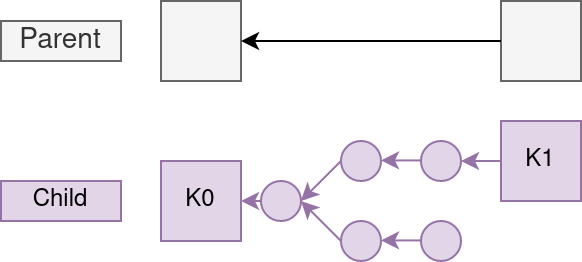
\includegraphics[scale=0.35]{microfork}
\end{figure}

\subsubsection{Generational forks}

This kind of attack is not a problem in PoW based BitcoinNG as producing
keyblocks is a hard task. On the contrary keyblocks on hyperchains are really,
really cheap - a malicious leader might flood the network with conflicting
keyblocks:

\begin{figure}[h]
	\caption{Generational Fork}
	\centering
	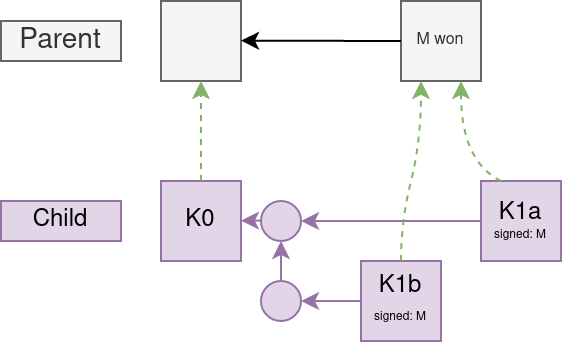
\includegraphics[scale=0.35]{genfork}
\end{figure}

The $K1a$, $K1b$, etc. are keyblocks on the child chain emitted by a malicious
leader over different microblocks. This
effectively splits the network in many parts, as it becomes unclear to which of
the forks the delegates should commit. To resolve this issue, a single leader
must be agreed upon using some additional mechanism – a new election
should be performed with the exclusion of the compromised delegate.

To notify the network about the generational fork, the peers need to announce
this fact on the parent chain by publishing the fraud commitments and the
cryptographic proofs of generational fraud (PoGF). Each commitment has to point to
the latest child keyblock considered by the delegates to be
valid, that is the generation where the fork starts. The committer also needs
to submit to which fork they want to contribute – if they get elected they
will keep building on it (we disallow rollbacks). The voting power should be
calculated based on the latest block before the fraud was detected.


\begin{figure}[h]
	\caption{Generational Fork Solving}
	\centering
	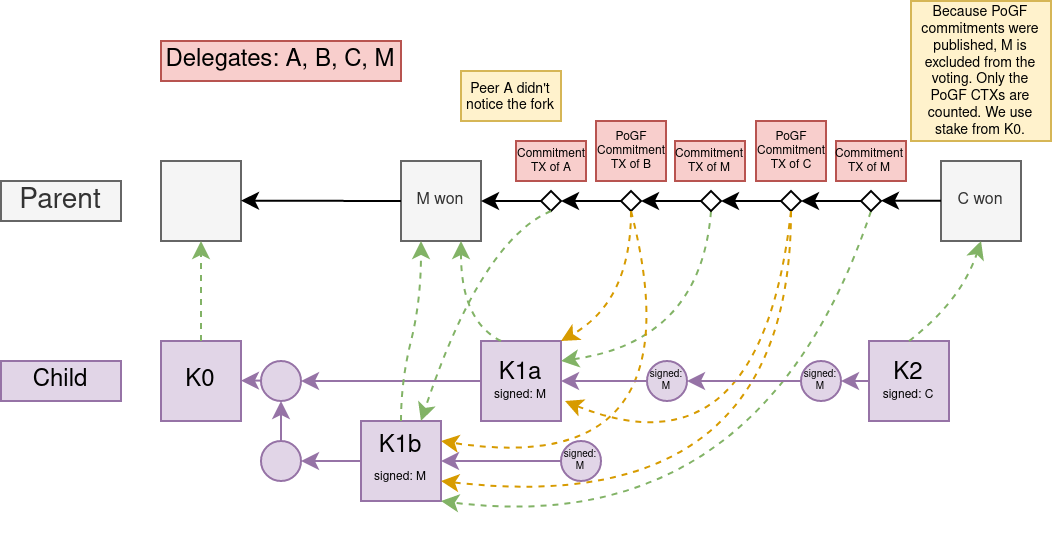
\includegraphics[scale=0.35]{genfraud}
\end{figure}

Due to network propagation
delays and connectivity failures, some nodes might not notice that a generational
fork was created and not respond accordingly. New nodes or the ones catching up
after downtime need to be aware that a generational fork was created and apply
the appropriate resolution. Some of them may commit to one of the forks and receive a fraud
notification after they started mining. Therefore, we introduce a metric over the
branches that we are going to call "difficulty" for a conventional reason. The
rule to resolve conflicts caused by such data races is similar to already
existing PoW strategy "follow the most difficult chain," and the formula goes
as follows:
\begin{minipage}{\linewidth}
\begin{lstlisting}
  difficulty : Block -> Int
  difficulty(Genesis) = 0
  difficulty(block) =
    if exists proof of generational fraud on /block/
    then sum of the voting power of delegates
           that committed to /prev(block)/ +
         sum of the voting power of delegates
           that committed to solve the genfork
    else sum of the voting power of delegates
           that committed to /prev(block)/
\end{lstlisting}
\end{minipage}

If two forks have the same difficulty, then we prefer the one with lower
block hash. This formula ensures that keyblocks pointing to a PoGF are always
strongly preferred over ordinary keyblocks – delegates who detect generational
forks have higher priority over poorly connected/bootstrapping/syncing ones.

This solution may look vulnerable to situations where the leader doesn't respond
or responds with significant delay. To solve these cases, we just elect a new
leader, stalling the network for a while. To vanish the doubts arising when the
previous leader reappears, we can assume
finalization after $f$ (implementation dependent) generations.

There is a compelling case where the malicious leader submits a generational
fork by publishing keyblocks on conflicting microblocks.
Here we want to prioritize PoGF because the consequences of the forks on
keyblocks are much more severe than these on microblocks, and we would need to
solve them anyway.

\subsection{Stake grinding}

Since the RNG depends ultimately on the keyblock hash on the PoW chain, it is
impossible to predict its outcomes. One could try to mine the parent chain
in a special way, but it would require so much computational power that in
most cases it would be easier to take control over it by some 51\% attack.

\subsection{Long range attack}
While it is still possible to perform it, it would be impossible to do it in
silence and without preparation since the very beginning. The commitments
guarantee that the information of the delegates is stored on an immutable chain,
and one would need to announce their will of mining some suspicious blocks during
the full period of the attack. This would quickly expose the intention of the attacker
and let the others prepare for an eventual surprise (by blacklisting them, for example).

\subsection{Avoiding punishments}
Depending on the circumstances on the network the transaction fees may vary
– this makes the original penalty system from BitcoinNG not sufficient in every
case as the risk of fraud detection may be much lesser than expected profit.

One of the most natural ideas is to freeze the stake with some period before the
election. In this scenario, the protocol will be able to painfully slash the
malicious leaders by burning/redistributing their stake. However, this may raise
some problems when the delegated voting is used – the malicious leader may vote
for their second, empty account that will do the fraud losing potentially
nothing in case of getting compromised. This scenario can be dealt with, allowing only
top $k$ stakers to be voted on or slashing \textit{everyone} who supported the
malicious leader. We leave this implementation-dependent as different solutions
require different security approaches.
